\documentclass{standalone}
\usepackage{tikz}
\usetikzlibrary{patterns, positioning}
\usepackage[sfdefault]{ClearSans} %% option 'sfdefault' activates Clear Sans as the default text font
\usepackage[T1]{fontenc}

\begin{document}
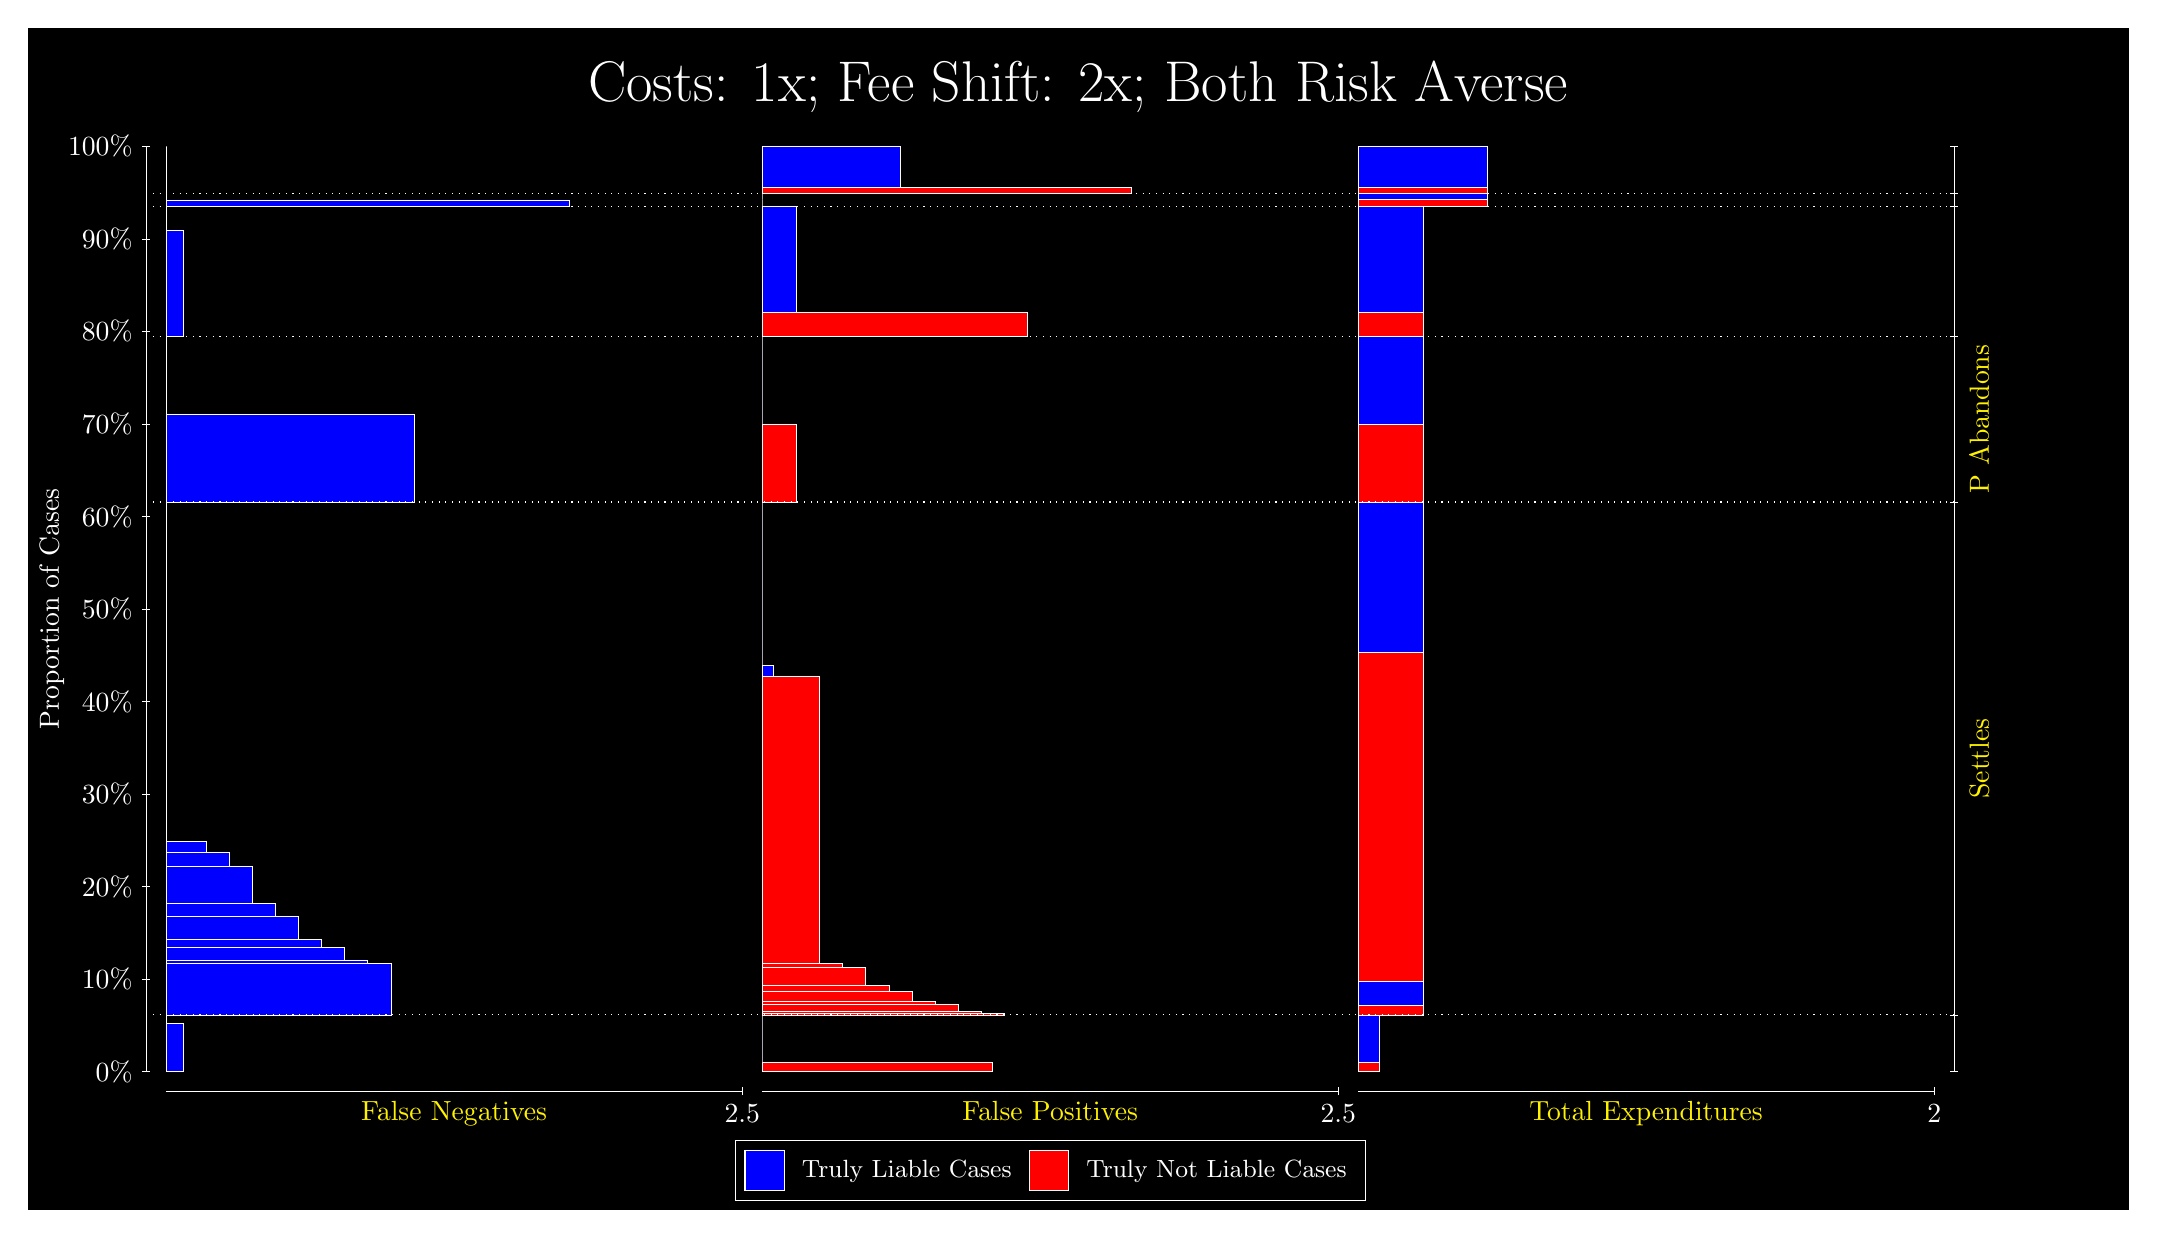
\begin{tikzpicture}
\draw[fill=black] (0,0) rectangle (26.667,15);
\draw[text=white] (0,13.5) rectangle (26.667,15) node[midway] {\huge Costs: 1x; Fee Shift: 2x; Both Risk Averse};
\draw[white, very thin] (1.5,1.75) -- (1.5,13.5);
\node[rotate=90, text=white, anchor=center] at (0.3, 7.625) {Proportion of Cases};
\draw[white, very thin] (1.45,1.75) -- (1.55,1.75);
\node[text=white, anchor=east] at (1.45, 1.75) {0\%};
\draw[white, very thin] (1.45,2.925) -- (1.55,2.925);
\node[text=white, anchor=east] at (1.45, 2.925) {10\%};
\draw[white, very thin] (1.45,4.1) -- (1.55,4.1);
\node[text=white, anchor=east] at (1.45, 4.1) {20\%};
\draw[white, very thin] (1.45,5.275) -- (1.55,5.275);
\node[text=white, anchor=east] at (1.45, 5.275) {30\%};
\draw[white, very thin] (1.45,6.45) -- (1.55,6.45);
\node[text=white, anchor=east] at (1.45, 6.45) {40\%};
\draw[white, very thin] (1.45,7.625) -- (1.55,7.625);
\node[text=white, anchor=east] at (1.45, 7.625) {50\%};
\draw[white, very thin] (1.45,8.8) -- (1.55,8.8);
\node[text=white, anchor=east] at (1.45, 8.8) {60\%};
\draw[white, very thin] (1.45,9.975) -- (1.55,9.975);
\node[text=white, anchor=east] at (1.45, 9.975) {70\%};
\draw[white, very thin] (1.45,11.15) -- (1.55,11.15);
\node[text=white, anchor=east] at (1.45, 11.15) {80\%};
\draw[white, very thin] (1.45,12.325) -- (1.55,12.325);
\node[text=white, anchor=east] at (1.45, 12.325) {90\%};
\draw[white, very thin] (1.45,13.5) -- (1.55,13.5);
\node[text=white, anchor=east] at (1.45, 13.5) {100\%};

\draw[white, very thin] (24.457,1.75) -- (24.457,13.5);
\draw[white, very thin] (24.407,1.75) -- (24.507,1.75);
\node[anchor=west] at (24.407, 1.75) {};
\draw[white, very thin] (24.407,2.4702) -- (24.507,2.4702);
\node[anchor=west] at (24.407, 2.4702) {};
\draw[white, very thin] (24.407,8.9833) -- (24.507,8.9833);
\node[anchor=west] at (24.407, 8.9833) {};
\draw[white, very thin] (24.407,11.084) -- (24.507,11.084);
\node[anchor=west] at (24.407, 11.084) {};
\draw[white, very thin] (24.407,12.735) -- (24.507,12.735);
\node[anchor=west] at (24.407, 12.735) {};
\draw[white, very thin] (24.407,12.904) -- (24.507,12.904);
\node[anchor=west] at (24.407, 12.904) {};
\draw[white, very thin] (24.407,13.5) -- (24.507,13.5);
\node[anchor=west] at (24.407, 13.5) {};

\draw[white, very thin, fill=blue] (1.75,1.75) rectangle (1.9696,2.3589);
\draw[white, very thin, fill=red] (1.75,2.3589) rectangle (1.75,2.4702);
\draw[white, very thin, fill=blue] (1.75,2.4702) rectangle (4.6044,3.1262);
\draw[white, very thin, fill=blue] (1.75,3.1262) rectangle (4.3116,3.1633);
\draw[white, very thin, fill=blue] (1.75,3.1633) rectangle (4.0188,3.3292);
\draw[white, very thin, fill=blue] (1.75,3.3292) rectangle (3.7261,3.432);
\draw[white, very thin, fill=blue] (1.75,3.432) rectangle (3.4333,3.7212);
\draw[white, very thin, fill=blue] (1.75,3.7212) rectangle (3.1406,3.8912);
\draw[white, very thin, fill=blue] (1.75,3.8912) rectangle (2.8478,4.3549);
\draw[white, very thin, fill=blue] (1.75,4.3549) rectangle (2.5551,4.5399);
\draw[white, very thin, fill=blue] (1.75,4.5399) rectangle (2.2623,4.6805);
\draw[white, very thin, fill=red] (1.75,4.6805) rectangle (1.75,8.9833);
\draw[white, very thin, fill=blue] (1.75,8.9833) rectangle (4.8971,10.098);
\draw[white, very thin, fill=red] (1.75,10.098) rectangle (1.75,11.084);
\draw[white, very thin, fill=blue] (1.75,11.084) rectangle (1.9696,12.432);
\draw[white, very thin, fill=red] (1.75,12.432) rectangle (1.75,12.735);
\draw[white, very thin, fill=blue] (1.75,12.735) rectangle (6.8732,12.814);
\draw[white, very thin, fill=red] (1.75,12.814) rectangle (1.75,12.904);
\draw[white, very thin, fill=red] (1.75,12.904) rectangle (1.75,12.985);
\draw[white, very thin, fill=blue] (1.75,12.985) rectangle (1.75,13.5);
\draw[white, very thin, fill=red] (9.3189,1.75) rectangle (12.246,1.8613);
\draw[white, very thin, fill=blue] (9.3189,1.8613) rectangle (9.3189,2.4702);
\draw[white, very thin, fill=red] (9.3189,2.4702) rectangle (12.393,2.4878);
\draw[white, very thin, fill=red] (9.3189,2.4878) rectangle (12.1,2.5193);
\draw[white, very thin, fill=red] (9.3189,2.5193) rectangle (11.807,2.6012);
\draw[white, very thin, fill=red] (9.3189,2.6012) rectangle (11.515,2.6401);
\draw[white, very thin, fill=red] (9.3189,2.6401) rectangle (11.222,2.7634);
\draw[white, very thin, fill=red] (9.3189,2.7634) rectangle (10.929,2.7675);
\draw[white, very thin, fill=red] (9.3189,2.7675) rectangle (10.929,2.8454);
\draw[white, very thin, fill=red] (9.3189,2.8454) rectangle (10.636,3.0803);
\draw[white, very thin, fill=red] (9.3189,3.0803) rectangle (10.344,3.1195);
\draw[white, very thin, fill=red] (9.3189,3.1195) rectangle (10.051,6.7731);
\draw[white, very thin, fill=blue] (9.3189,6.7731) rectangle (9.4652,6.9136);
\draw[white, very thin, fill=blue] (9.3189,6.9136) rectangle (9.3189,8.9833);
\draw[white, very thin, fill=red] (9.3189,8.9833) rectangle (9.758,9.9702);
\draw[white, very thin, fill=blue] (9.3189,9.9702) rectangle (9.3189,11.084);
\draw[white, very thin, fill=red] (9.3189,11.084) rectangle (12.686,11.387);
\draw[white, very thin, fill=blue] (9.3189,11.387) rectangle (9.758,12.735);
\draw[white, very thin, fill=red] (9.3189,12.735) rectangle (9.3189,12.825);
\draw[white, very thin, fill=blue] (9.3189,12.825) rectangle (9.3189,12.904);
\draw[white, very thin, fill=red] (9.3189,12.904) rectangle (14.003,12.985);
\draw[white, very thin, fill=blue] (9.3189,12.985) rectangle (11.075,13.5);
\draw[white, very thin, fill=red] (16.888,1.75) rectangle (17.162,1.8613);
\draw[white, very thin, fill=blue] (16.888,1.8613) rectangle (17.162,2.4702);
\draw[white, very thin, fill=red] (16.888,2.4702) rectangle (17.711,2.5976);
\draw[white, very thin, fill=blue] (16.888,2.5976) rectangle (17.711,2.9001);
\draw[white, very thin, fill=red] (16.888,2.9001) rectangle (17.711,7.0755);
\draw[white, very thin, fill=blue] (16.888,7.0755) rectangle (17.711,8.9833);
\draw[white, very thin, fill=red] (16.888,8.9833) rectangle (17.711,9.9702);
\draw[white, very thin, fill=blue] (16.888,9.9702) rectangle (17.711,11.084);
\draw[white, very thin, fill=red] (16.888,11.084) rectangle (17.711,11.387);
\draw[white, very thin, fill=blue] (16.888,11.387) rectangle (17.711,12.735);
\draw[white, very thin, fill=red] (16.888,12.735) rectangle (18.534,12.825);
\draw[white, very thin, fill=blue] (16.888,12.825) rectangle (18.534,12.904);
\draw[white, very thin, fill=red] (16.888,12.904) rectangle (18.534,12.985);
\draw[white, very thin, fill=blue] (16.888,12.985) rectangle (18.534,13.5);
\draw[white, dotted] (1.5,2.4702) -- (24.457,2.4702);
\draw[white, dotted] (1.5,8.9833) -- (24.457,8.9833);
\draw[white, dotted] (1.5,11.084) -- (24.457,11.084);
\draw[white, dotted] (1.5,12.735) -- (24.457,12.735);
\draw[white, dotted] (1.5,12.904) -- (24.457,12.904);
\draw[white, very thin] (1.75,1.5) -- (9.0689,1.5);
\node[text=yellow, anchor=north] at (5.4094, 1.5) {False Negatives};
\draw[white, very thin] (9.0689,1.45) -- (9.0689,1.55);
\node[text=white, anchor=north] at (9.0689, 1.45) {2.5};

\draw[white, very thin] (9.3189,1.5) -- (16.638,1.5);
\node[text=yellow, anchor=north] at (12.978, 1.5) {False Positives};
\draw[white, very thin] (16.638,1.45) -- (16.638,1.55);
\node[text=white, anchor=north] at (16.638, 1.45) {2.5};

\draw[white, very thin] (16.888,1.5) -- (24.207,1.5);
\node[text=yellow, anchor=north] at (20.547, 1.5) {Total Expenditures};
\draw[white, very thin] (24.207,1.45) -- (24.207,1.55);
\node[text=white, anchor=north] at (24.207, 1.45) {2};


\node[text=yellow, centered, rotate=90] at (24.777, 5.7268) {Settles};
\node[text=yellow, centered, rotate=90] at (24.777, 10.034) {P Abandons};




\draw (12.978300999999998,1.5) node[draw=none] (baseCoordinate) {};
\begin{scope}[align=center]
        \matrix[scale=0.5, draw=white, below=0.5cm of baseCoordinate, nodes={draw}, column sep=0.1cm]{
            \node[rectangle, draw, minimum width=0.5cm, minimum height=0.5cm, fill=blue] {}; &
            \node[draw=none, font=\small, text=white] (B) {Truly Liable Cases}; &
            \node[rectangle, draw, minimum width=0.5cm, minimum height=0.5cm, fill=red] {}; &
            \node[draw=none, font=\small, text=white] (B) {Truly Not Liable Cases}; \\
            };
\end{scope}

\end{tikzpicture}
\end{document}